\documentclass[11pt,twoside,openright]{book}

\usepackage{styles/rbruacademic}

\begin{document}

% -------------------------------------------------------------
% หน้าปก 3D Pixar Semi-realistics & XeLaTeX TikZ Transparent Architecture
% -------------------------------------------------------------
\begin{titlepage}
\thispagestyle{empty}
\begingroup
\setlength{\XeTeXlinebreakskip}{0pt}
\begin{tikzpicture}[remember picture, overlay]
    % 1. Full-Bleed 3D Pixar Cover Artwork (6x9 inch)
    \node[anchor=center, inner sep=0pt] at (current page.center) {
        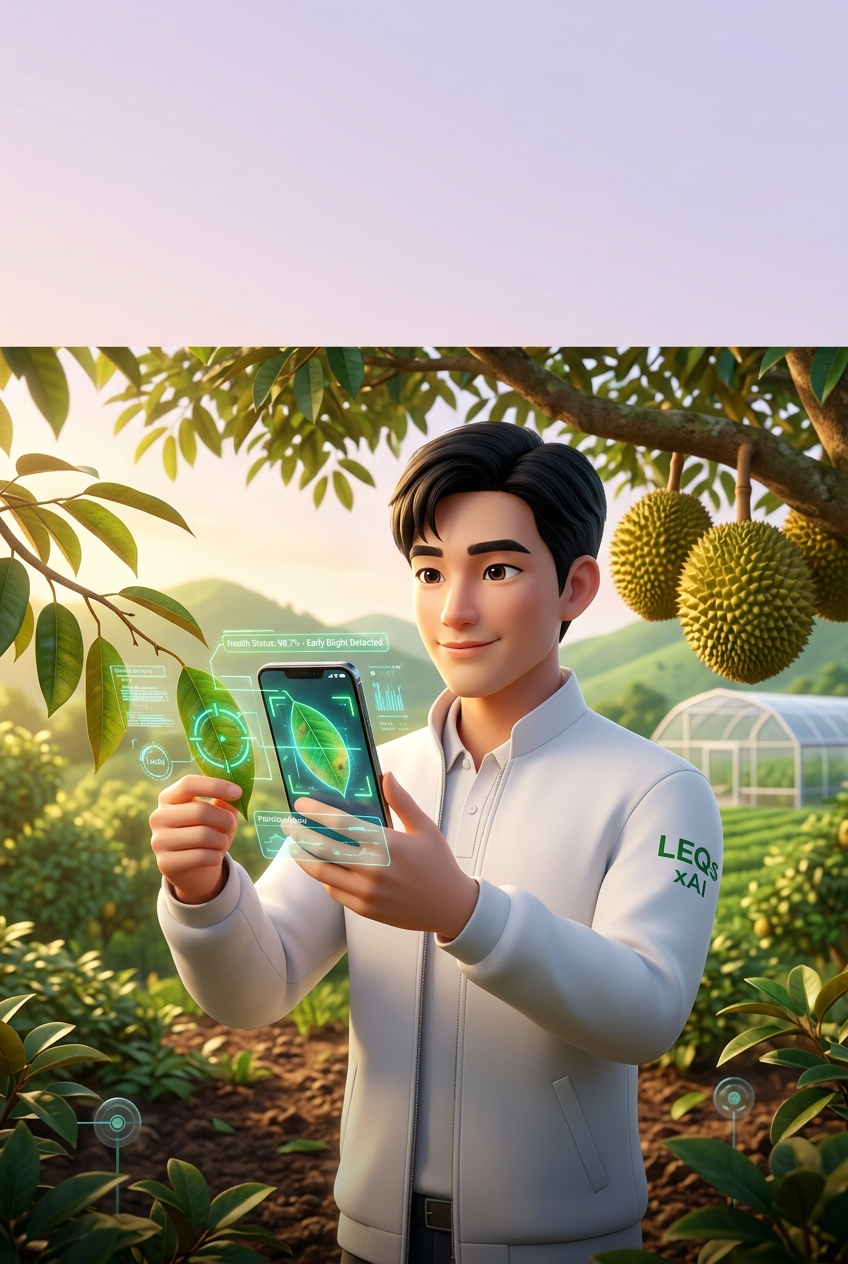
\includegraphics[width=\paperwidth,height=\paperheight]{figures/cover_art.jpg}
    };

    % 2. UPPER SKY ZONE: Dual-Layer Micro Drop-Shadow Typography
    % Category Badge
    \node[anchor=north, align=center] at ([yshift=-0.40in]current page.north) {
        {\fontsize{8.5}{11}\selectfont\bfseries\color{white} SMART AGRICULTURE \& COMPUTER VISION SERIES}\\[2pt]
        {\fontsize{8}{10}\selectfont\color{yellow!90!white} เอกสารคำสอนและคู่มือปฏิบัติการขั้นสูง \textbullet\ มหาวิทยาลัยราชภัฏรำไพพรรณี}
    };

    % Main Title Line 1 (Shadow layer)
    \node[anchor=north, align=center, text width=5.2in] at ([xshift=0.6pt, yshift=-0.70in]current page.north) {
        {\fontsize{18}{22}\selectfont\bfseries\color{white} แอปพลิเคชันสมาร์ทโฟนตรวจวิเคราะห์โรค}\\
        {\fontsize{22}{27}\selectfont\bfseries\color{white} และวินิจฉัยโรคใบทุเรียนด้วยปัญญาประดิษฐ์}
    };
    % Main Title Line 1 (Foreground layer)
    \node[anchor=north, align=center, text width=5.2in] at ([yshift=-0.71in]current page.north) {
        {\fontsize{18}{22}\selectfont\bfseries\color{rbruNavy!95!black} แอปพลิเคชันสมาร์ทโฟนตรวจวิเคราะห์โรค}\\
        {\fontsize{22}{27}\selectfont\bfseries\color{agriGreen!95!black} และวินิจฉัยโรคใบทุเรียนด้วยปัญญาประดิษฐ์}
    };

    % English Subtitle
    \node[anchor=north, align=center] at ([yshift=-1.40in]current page.north) {
        {\fontsize{8.5}{11}\selectfont\bfseries\color{rbruNavy!90} EDGE AI SMARTPHONE APPLICATION FOR DURIAN LEAF PATHOLOGY \& DIAGNOSTICS}
    };

    % 3. BOTTOM SOIL ZONE: Natural Dark Canvas for Author Metadata
    % Shadow layer
    \node[anchor=south, align=center, text width=5.2in] at ([xshift=0.6pt, yshift=0.30in]current page.south) {
        {\fontsize{13}{16}\selectfont\bfseries\color{black} ผู้ช่วยศาสตราจารย์ ดร.ชีวะ ทัศนา}
    };
    % Foreground layer
    \node[anchor=south, align=center, text width=5.2in] at ([yshift=0.31in]current page.south) {
        {\fontsize{13}{16}\selectfont\bfseries\color{white} ผู้ช่วยศาสตราจารย์ ดร.ชีวะ ทัศนา}\\[3pt]
        {\fontsize{8.5}{11}\selectfont\color{white!95} ศูนย์วิจัยฟิสิกส์ดิจิทัลและปัญญาประดิษฐ์ทางการเกษตร คณะวิทยาศาสตร์และเทคโนโลยี}\\[2pt]
        {\fontsize{8}{10}\selectfont\color{yellow!90!white} มหาวิทยาลัยราชภัฏรำไพพรรณี \textbullet\ พ.ศ. 2569}
    };
\end{tikzpicture}
\endgroup
\end{titlepage}

\cleardoublepage

% -------------------------------------------------------------
% หน้าปกในเวกเตอร์ Dark Mode (Vector Inner Title Page)
% -------------------------------------------------------------
\thispagestyle{empty}
\pagecolor{black!94}
\begingroup
\setlength{\XeTeXlinebreakskip}{0pt}
\begin{tikzpicture}[remember picture, overlay]
    % วาดองค์ประกอบเวกเตอร์ TikZ ดิจิทัลฟาร์ม
    \draw[color=rbruGold!40, thick] ([yshift=-1.2in]current page.north) circle (0.65in);
    
    \node[anchor=center, align=center] at ([yshift=0.8in]current page.center) {
        {\fontsize{18}{22}\selectfont\bfseries\color{white} ระบบปัญญาประดิษฐ์วิเคราะห์โรคใบทุเรียน}\\[6pt]
        {\fontsize{12}{15}\selectfont\color{rbruGold} DURIAN LEAF DISEASE COMPUTER VISION SYSTEM}\\[14pt]
        {\color{rbruGold!70}\rule{0.6\textwidth}{1pt}}
    };

    \node[anchor=center, align=center] at ([yshift=-1.0in]current page.center) {
        {\fontsize{11}{14}\selectfont\color{white!90} ผู้ช่วยศาสตราจารย์ ดร.ชีวะ ทัศนา}\\[4pt]
        {\fontsize{9}{12}\selectfont\color{white!70} สาขาวิชาฟิสิกส์และปัญญาประดิษฐ์ คณะวิทยาศาสตร์และเทคโนโลยี}\\[2pt]
        {\fontsize{8.5}{11}\selectfont\color{rbruGold!90} มหาวิทยาลัยราชภัฏรำไพพรรณี}
    };
\end{tikzpicture}
\endgroup
\newpage
\pagecolor{white}
\cleardoublepage

% -------------------------------------------------------------
% Frontmatter: คำนำ, สารบัญ
% -------------------------------------------------------------
\frontmatter
\chapter*{คำนำ}
\addcontentsline{toc}{chapter}{คำนำ}

เอกสารคำสอนและคู่มือวิชาการฉบับนี้ จัดทำขึ้นเพื่อรวบรวมองค์ความรู้ด้านการบูรณาการเทคโนโลยีคอมพิวเตอร์วิทัศน์ (\textbf{Computer Vision}) และการเรียนรู้เชิงลึก (\textbf{Deep Learning}) เข้ากับงานพยาธิวิทยาพืช (\textbf{Plant Pathology}) โดยมุ่งเน้นการแก้ปัญหาโรคใบทุเรียนซึ่งเป็นพืชเศรษฐกิจหลักของภาคตะวันออกและประเทศไทย

เนื้อหาในเล่มนี้ครอบคลุมตั้งแต่การคัดเลือกสถาปัตยกรรมโมเดลที่มีประสิทธิภาพสูงแต่น้ำหนักเบาอย่าง MobileNetV3, การสร้างไปป์ไลน์การจำแนกภาพแบบ End-to-End บน Google Colab และ PyTorch, การเพิ่มความโปร่งใสตรวจสอบได้ของปัญญาประดิษฐ์ด้วยเทคนิค Grad-CAM, ตลอดจนการแปลงโมเดลให้อยู่ในมาตรฐาน ONNX เพื่อนำไปติดตั้งบนอุปกรณ์ขอบ (Edge AI) และสมาร์ทโฟนของเกษตรกร

ผู้เขียนหวังเป็นอย่างยิ่งว่า เอกสารฉบับนี้จะเป็นประโยชน์ต่อนักศึกษา นักวิจัย เกษตรกร และผู้สนใจในการพัฒนานวัตกรรมเกษตรอัจฉริยะอย่างยั่งยืน

\vspace{1.5cm}
\begin{flushright}
\textbf{ผู้ช่วยศาสตราจารย์ ดร.ชีวะ ทัศนา}\\
มหาวิทยาลัยราชภัฏรำไพพรรณี
\end{flushright}

\clearpage
\tableofcontents
\clearpage
\listoftables
\clearpage
\listoffigures
\clearpage

% -------------------------------------------------------------
% Mainmatter: บทเนื้อหา
% -------------------------------------------------------------
\mainmatter
\chapter{วิทยาการโรคใบทุเรียนและสถาปัตยกรรมเกษตรอัจฉริยะ}
\label{chap:durian_pathology_ai}
\index{โรคใบทุเรียน}
\index{เกษตรอัจฉริยะ}
\index{Edge AI}

\section*{แผนบริหารการสอนประจำบทที่ 1}
\addcontentsline{toc}{section}{แผนบริหารการสอนประจำบทที่ 1}

\begin{planbox}{หัวข้อเนื้อหาประจำบท (Lesson Topics)}
\begin{enumerate}[leftmargin=1.5em, itemsep=2pt]
    \item ความสำคัญทางเศรษฐกิจของทุเรียนและปัญหาการระบาดของโรคทางใบ
    \item สัณฐานวิทยาและชีววิทยาของเชื้อสาเหตุโรคใบทุเรียนสำคัญ 3 ชนิด
    \item ปัจจัยทางจุลภูมิอากาศ (Microclimate) และวงจรระบาดวิทยาในแปลงปลูก
    \item สถาปัตยกรรมระบบเกษตรอัจฉริยะและการประมวลผลบนอุปกรณ์ขอบ (Edge AI Paradigm)
    \item ความท้าทายในการตรวจจับรอยโรคในสภาพแปลงเปิด (Field Operational Challenges)
    \item โค้ดตัวอย่าง: สคริปต์วิเคราะห์ความสัมพันธ์ระหว่างสภาพอากาศและการระบาดของโรค
    \item กรณีศึกษาการประยุกต์ใช้งานจริงในแปลงทดลองจังหวัดจันทบุรี
\end{enumerate}
\end{planbox}

\begin{planbox}{วัตถุประสงค์เชิงพฤติกรรม (Behavioral Objectives)}
เมื่อศึกษาบทที่ 1 จบแล้ว ผู้เรียนและผู้อ่านสามารถ:
\begin{enumerate}[leftmargin=1.5em, itemsep=2pt]
    \item อธิบายชีววิทยาและลักษณะรอยโรคของเชื้อสาเหตุทั้ง 3 กลุ่มได้อย่างถูกต้องตามหลักวิชาการ
    \item วิเคราะห์ความสัมพันธ์ระหว่างความชื้นสัมพัทธ์ อุณหภูมิ และการงอกของสปอร์เชื้อราก่อโรคได้
    \item เปรียบเทียบข้อดีและข้อจำกัดของระบบประมวลผลบนคลาวด์เทียบกับระบบ Edge AI บนสมาร์ทโฟนได้
    \item ออกแบบแผนการตรวจสำรวจแปลงทุเรียนด้วยเทคโนโลยีคอมพิวเตอร์วิทัศน์ได้อย่างมีประสิทธิภาพ
\end{enumerate}
\end{planbox}

\begin{planbox}{กิจกรรมการเรียนการสอน (Instructional Activities)}
\begin{enumerate}[leftmargin=1.5em, itemsep=2pt]
    \item การบรรยายเชิงทฤษฎีพยาธิวิทยาพืชเขตร้อนและกรอบแนวคิดปัญญาประดิษฐ์ทางการเกษตร
    \item การสังเกตและจำแนกตัวอย่างใบจริงที่แสดงอาการโรคใบจุดสาหร่าย โรคใบติด และโรคใบจุด
    \item การฝึกวิเคราะห์ข้อมูลเซนเซอร์สิ่งแวดล้อมแปลงปลูกด้วยภาษา Python เพื่อพยากรณ์ความเสี่ยง
    \item การอภิปรายกลุ่มย่อยเกี่ยวกับการนำเทคโนโลยีปัญญาประดิษฐ์ไปถ่ายทอดสู่เกษตรกรในพื้นที่
\end{enumerate}
\end{planbox}

\begin{planbox}{สื่อการเรียนการสอน (Instructional Media)}
\begin{enumerate}[leftmargin=1.5em, itemsep=2pt]
    \item สไลด์มัลติมีเดียแสดงลักษณะทางพยาธิวิทยาของเซลล์ใบและโครงข่ายการระบาด
    \item คลังข้อมูลและภาพถ่ายตัวอย่างใบจริงความละเอียดสูงจากแปลงปลูกภาคตะวันออก
    \item สคริปต์ภาษา Python สำหรับจำลองสมการการเจริญเติบโตของประชากรเชื้อก่อโรค
\end{enumerate}
\end{planbox}

\begin{planbox}{การวัดและประเมินผล (Assessment \& Evaluation)}
\begin{enumerate}[leftmargin=1.5em, itemsep=2pt]
    \item แบบทดสอบวัดความรู้เชิงทฤษฎีพยาธิวิทยาและสถาปัตยกรรมระบบ Edge AI (40\%)
    \item ความถูกต้องของผลงานการวิเคราะห์ชุดข้อมูลสภาพแวดล้อมด้วย Python (40\%)
    \item การนำเสนอรายงานกรณีศึกษาและคุณภาพการตอบคำถามทบทวนท้ายบท (20\%)
\end{enumerate}
\end{planbox}

\clearpage

\section{บริบททางเศรษฐกิจและปัญหาโรคใบทุเรียนในประเทศไทย}
\index{ทุเรียนหมอนทอง}
\index{พยาธิวิทยาพืช}

ทุเรียน (\textit{Durio zibethinus} L.) ได้รับการขนานนามว่าเป็นราชาแห่งผลไม้ (King of Fruits) และถือเป็นพืชเศรษฐกิจที่สร้างมูลค่าการส่งออกสูงสุดให้แก่ประเทศไทย โดยเฉพาะอย่างยิ่งในเขตภาคตะวันออก ได้แก่ จังหวัดจันทบุรี ระยอง และตราด พันธุ์การค้าที่สำคัญที่สุดคือพันธุ์หมอนทอง ซึ่งมีความอ่อนไหวต่อสภาพภูมิอากาศและความชื้นสูงเป็นพิเศษ ในช่วงฤดูมรสุมที่มีฝนตกชุกต่อเนื่อง สภาพแวดล้อมในทรงพุ่มทุเรียนจะมีความชื้นสัมพัทธ์สูงเกินกว่าร้อยละ 85 และอุณหภูมิเฉลี่ย 26--32 องศาเซลเซียส ซึ่งเป็นสภาวะที่เอื้ออำนวยอย่างยิ่งต่อการขยายพันธุ์และการงอกของสปอร์เชื้อราก่อโรคทางใบ

ความสมบูรณ์ของพื้นที่ใบ (Leaf Area Index: LAI) ถือเป็นดัชนีชี้วัดความสามารถในการสังเคราะห์ด้วยแสงและการสะสมอาหารสำหรับการออกดอกและติดผล หากใบทุเรียนได้รับความเสียหายจากรอยโรคเกินกว่าร้อยละ 20 ของทรงพุ่ม จะส่งผลกระทบให้ต้นทุเรียนเกิดภาวะเครียด สลัดดอกและผลอ่อน ส่งผลให้ผลผลิตลดลงมากกว่าร้อยละ 40 หรือในกรณีที่รุนแรง ต้นทุเรียนอาจทรุดโทรมและยืนต้นตายได้

\begin{table}[H]
\caption{กลุ่มโรคใบทุเรียนสำคัญ เชื้อสาเหตุ และผลกระทบต่อผลผลิตทางการเกษตร}
\label{tab:ch01_diseases_overview}
\begin{tabularx}{\textwidth}{L{2.4cm}L{3.4cm}L{3.8cm}Y}
\toprule
\textbf{กลุ่มโรคใบทุเรียน} & \textbf{เชื้อสาเหตุ (Pathogen)} & \textbf{ลักษณะรอยโรคบนใบ} & \textbf{ผลกระทบทางเศรษฐกิจ} \\
\midrule
โรคใบจุดสาหร่าย & สาหร่ายกาฝากเซลล์เดียว \textit{Cephaleuros virescens} & แผลจุดกลมฟูสีส้มอมเขียวคล้ายกำมะหยี่บนผิวใบ & บดบังแสงแดดสังเคราะห์อาหาร ใบเหลืองและร่วงก่อนกำหนด \\
\addlinespace
โรคใบติด (ราใบติด) & เชื้อราเส้นใยชั้นต่ำ \textit{Rhizoctonia solani} Kühn & แผลฉ่ำน้ำคล้ายน้ำร้อนลวก เส้นใยขาวโยงใบไหม้ติดกัน & ใบไหม้หลุดร่วงทั้งกิ่งอย่างรวดเร็ว กิ่งแห้งตาย ปริมาณผลผลิตร่วงหล่น \\
\addlinespace
โรคใบจุด/แอนแทรคโนส & เชื้อรา \textit{Colletotrichum gloeosporioides} & แผลไหม้สีน้ำตาลเข้ม มีวงซ้อนลายคลื่น จุดดำคอนิเดีย & เกิดแผลเนื้อเยื่อตาย ขอบใบไหม้ ทรงพุ่มโปร่ง ต้นชะงักการโต \\
\addlinespace
ใบปกติสมบูรณ์ & ปราศจากการเข้าทำลาย & แผ่นใบสีเขียวเข้ม ผิวมันวาว เส้นใบชัดเจน & สังเคราะห์แสงได้เต็มศักยภาพ ต้นสมบูรณ์พร้อมออกดอก \\
\bottomrule
\end{tabularx}
\end{table}

\section{ชีววิทยาและการระบาดของเชื้อสาเหตุทางใบ}
\index{Cephaleuros virescens}
\index{Rhizoctonia solani}
\index{Colletotrichum gloeosporioides}

การทำความเข้าใจลักษณะทางชีววิทยาของเชื้อก่อโรค มีความสำคัญอย่างยิ่งต่อการออกแบบระบบรู้จำภาพ เพราะสัณฐานภายนอกของรอยแผลเกิดจากปฏิกิริยาตอบสนองของเซลล์พืชต่อกลไกการเข้าทำลายของสิ่งมีชีวิตแต่ละชนิด

\subsection{โรคใบจุดสาหร่าย (Algal Leaf Spot)}
โรคนี้เกิดจากสาหร่ายสีเขียวที่มีคลอโรฟิลล์แต่ดำรงชีพแบบเบียนกึ่งกาฝาก \textit{Cephaleuros virescens} โดยเส้นสายสาหร่ายจะเจริญแทรกตัวใต้ชั้นคิวติเคิล (Subcuticular) ของใบพืช จากนั้นจะแทงก้านชูสปอร์แรงเจียม (Sporangiophore) สีส้มสดหรือสีน้ำตาลอมแดงโผล่ขึ้นมาเหนือผิวใบ ทำให้มองเห็นด้วยตาเปล่าเป็นจุดนูนฟูคล้ายกำมะหยี่ เมื่อมองผ่านระบบภาพถ่าย RGB รอยโรคนี้จะมีค่าสีเด่นในช่องสัญญาณสีแดงและสีเขียว (Red-Green balance) ที่ต่างจากเนื้อเยื่อพืชปกติ

\subsection{โรคใบติด (Leaf Blight / Rhizoctonia Blight)}
เกิดจากเชื้อรา \textit{Rhizoctonia solani} ซึ่งมักสะสมอยู่ในเศษซากพืชและดินใต้โคนต้น เมื่อได้รับละอองฝนสาดขึ้นสู่ใบ กิ่ง หรือมีลมพัดพา เส้นใยรา (Mycelium) ชนิดไม่มีผนังกั้นจะเจริญลุกลามอย่างรวดเร็ว ปล่อยเอนไซม์ Pectinase และ Cellulase ย่อยสลายผนังเซลล์พืช ทำให้เนื้อเยื่อใบยุบตัวเป็นแผลฉ่ำน้ำ (Water-soaked lesion) สีเขียวหม่นปนน้ำตาล จากนั้นใบจะแห้งเหี่ยวและมีเส้นใยใยแมงมุมโยงยึดใบที่อยู่ติดกันไว้ ทำให้มองเห็นเป็นกลุ่มใบไหม้แขวนติดอยู่กับกิ่ง

\subsection{โรคใบจุดสนิมและแอนแทรคโนส (Leaf Spot / Anthracnose)}
เกิดจากเชื้อรา \textit{Colletotrichum gloeosporioides} เชื้อราสร้างสปอร์แบบไม่อาศัยเพศ (Conidia) แพร่กระจายตามหยดน้ำฝน เมื่อตกบนใบจะสร้างอวัยวะเกาะติด (Appressorium) เจาะทะลุผิวใบ แผลเริ่มต้นเป็นจุดฉ่ำน้ำขนาดเล็ก จากนั้นขยายเป็นแผลวงกลมหรือรูปไข่สีน้ำตาลเทา มีวงสีน้ำตาลเข้มซ้อนกันเป็นชั้นๆ (Concentric rings) ขอบแผลมีแถบสีเหลืองล้อมรอบ (Chlorotic halo)

\section{สถาปัตยกรรมระบบเกษตรอัจฉริยะและการตรวจวินิจฉัยด้วย Edge AI}
\index{สถาปัตยกรรม Edge AI}
\index{ระบบโครงข่ายประสาท}

ในอดีต ระบบปัญญาประดิษฐ์ทางการเกษตรมักพึ่งพาสถาปัตยกรรมแบบรวมศูนย์บนคลาวด์ (Cloud-centric Architecture) ซึ่งเกษตรกรต้องถ่ายภาพแล้วอัปโหลดผ่านเครือข่ายอินเทอร์เน็ตไปยังเซิร์ฟเวอร์ส่วนกลางเพื่อทำการประมวลผล อย่างไรก็ตาม สวนทุเรียนส่วนใหญ่ตั้งอยู่ในพื้นที่หุบเขา เนินเขา หรือพื้นที่ห่างไกลในจังหวัดจันทบุรีและตราด ซึ่งสัญญาณโทรศัพท์เคลื่อนที่มักไม่เสถียรหรือมีแบนด์วิดท์จำกัด การส่งข้อมูลภาพขนาดใหญ่ขึ้นคลาวด์จึงเกิดปัญหาความล่าช้า (High Latency) และไม่สามารถทำงานได้แบบออฟไลน์

\begin{figure}[H]
\centering
\begin{tikzpicture}[
    node distance=1.5cm,
    font=\fontsize{9}{11}\selectfont,
    box/.style={draw=deepIndigo, fill=white, rounded corners=3mm, inner sep=6pt, align=center, thick, drop shadow},
    edgebox/.style={draw=neonEmerald!80!black, fill=agriLightGreen!50, rounded corners=3mm, inner sep=6pt, align=center, very thick, drop shadow},
    cloudbox/.style={draw=techAqua, fill=softCyanBg!40, rounded corners=3mm, inner sep=6pt, align=center, thick, drop shadow},
    arrow/.style={-{Stealth[length=3mm]}, thick, draw=deepIndigo}
]
    \node[box] (orchard) {\textbf{แปลงสวนทุเรียน (Durian Orchard)}\\ต้นทุเรียนจริง / สภาพแสงธรรมชาติ};
    \node[edgebox, right=1.2cm of orchard] (mobile) {\textbf{อุปกรณ์ขอบ (Edge Device)}\\สมาร์ทโฟน / กล้องพกพา\\MobileNetV3 ONNX Engine\\\textbf{[Offline Inference $<20$ ms]}};
    \node[edgebox, below=1.0cm of mobile] (xai) {\textbf{ระบบตีความรอยโรค}\\\textbf{Explainable AI (Grad-CAM)}\\แผนที่ความร้อนชี้ตำแหน่งแผล};
    \node[cloudbox, right=1.2cm of mobile] (cloud) {\textbf{ระบบคลาวด์ส่วนกลาง}\\\textbf{Cloud Management CMS}\\บันทึกพิกัด GPS / ระดับความรุนแรง\\รายงานสถิติแปลงใหญ่};

    \draw[arrow] (orchard) -- node[above, font=\fontsize{7.5}{9.5}\selectfont] {ภาพถ่ายสด} (mobile);
    \draw[arrow] (mobile) -- (xai);
    \draw[arrow, dashed] (mobile) -- node[above, font=\fontsize{7.5}{9.5}\selectfont] {ซิงก์เมื่อมีเน็ต} (cloud);
    \draw[arrow] (xai) -| node[below, pos=0.25, font=\fontsize{7.5}{9.5}\selectfont] {คำแนะนำเกษตรกร} (orchard);
\end{tikzpicture}
\caption{สถาปัตยกรรมบูรณาการระบบ Edge AI ตรวจวิเคราะห์โรคใบทุเรียนแบบออฟไลน์ในแปลงเกษตร}
\label{fig:ch01_aiot_edge_paradigm}
\end{figure}

การเปลี่ยนผ่านสู่แนวคิด \textbf{Edge AI} โดยการนำโมเดลโครงข่ายประสาทเทียมขนาดกะทัดรัดที่ผ่านการปรับแต่งอย่างเหมาะสม (Model Optimization) มาฝังไว้ในตัวสมาร์ทโฟนของเกษตรกรโดยตรง ทำให้ระบบสามารถวินิจฉัยโรคได้ทันทีที่เล็งกล้องไปยังใบพืช ด้วยความเร็วระดับ 30 เฟรมต่อวินาที (Real-time Video Inference) โดยไม่ต้องพึ่งพาสัญญาณอินเทอร์เน็ตแม้แต่น้อย

\section{ปฏิทินการระบาดตามฤดูกาลและมาตรการเฝ้าระวังเชิงรุก}
\index{ปฏิทินการระบาด}
\index{ระบาดวิทยาตามฤดูกาล}

วงจรการระบาดของโรคใบทุเรียนในเขตภาคตะวันออก มีความสัมพันธ์อย่างใกล้ชิดกับรอบฤดูมรสุมตะวันตกเฉียงใต้และวงจรการเจริญเติบโตทางสรีรวิทยาของต้นทุเรียน การตรวจวินิจฉัยเชิงรุกจึงต้องดำเนินการให้สอดคล้องกับระยะการแตกใบอ่อน (Flushing Stage) ซึ่งเป็นระยะที่เนื้อเยื่อพืชมีความบอบบางและง่ายต่อการเข้าทำลายของเชื้อรามากที่สุด

\begin{table}[H]
\caption{ปฏิทินระบาดวิทยาของโรคใบทุเรียนและระดับความเสี่ยงในรอบปีการผลิตภาคตะวันออก}
\label{tab:ch01_seasonal_calendar}
\begin{tabularx}{\textwidth}{L{2.5cm}L{3.4cm}L{2.6cm}Y}
\toprule
\textbf{ช่วงเดือน} & \textbf{ระยะการเติบโตของทุเรียน} & \textbf{สภาพภูมิอากาศ} & \textbf{โรคสำคัญและระดับความเสี่ยง} \\
\midrule
พ.ค. -- มิ.ย. & ฟื้นฟูต้นหลังเก็บเกี่ยว / ใบอ่อนชุดที่ 1 & ฝนเริ่มตกชุก RH $> 80\%$ & โรคใบติด (ปานกลาง), โรคใบจุดสาหร่าย (เริ่มต้น) \\
\addlinespace
ก.ค. -- ส.ค. & แตกใบอ่อนชุดที่ 2 / สะสมอาหาร & มรสุมหนัก ฝนตกชุกต่อเนื่อง & \textbf{โรคใบติด (วิกฤตสูงสุด)}, แอนแทรคโนส (สูง) \\
\addlinespace
ก.ย. -- ต.ค. & ใบเพสลาดพร้อมสะสมตาดอก & ฝนตกชุกสลับแดดจัด & โรคใบจุดสาหร่าย (สูงสุด), โรคใบจุด (สูง) \\
\addlinespace
พ.ย. -- ธ.ค. & ระยะพัฒนาตาดอก / ดอกบาน & ลมหนาว อากาศเริ่มแห้ง & โรคราแป้งและเพลี้ยไฟ (ใบแก่ทนทานต่อราใบติด) \\
\bottomrule
\end{tabularx}
\end{table}

จากตารางที่ \ref{tab:ch01_seasonal_calendar} ช่วงเดือนกรกฎาคมถึงตุลาคมถือเป็นช่วงเวลาวิกฤตสูงสุดที่เกษตรกรจำเป็นต้องนำระบบ AI บนสมาร์ทโฟนออกสำรวจแปลงอย่างสม่ำเสมออย่างน้อยสัปดาห์ละ 2 ครั้ง เพื่อตรวจจับรอยโรคตั้งแต่ระยะแผลขนาดเล็กก่อนที่จะลุกลามไหม้ทั้งกิ่ง

\section{ความท้าทายในการตรวจจับรอยโรคในสภาพแปลงเปิด}
\index{สภาพแวดล้อมแปลงเปิด}

การนำคอมพิวเตอร์วิทัศน์มาใช้กับงานพืชสวนมีความซับซ้อนกว่าภาพถ่ายในห้องปฏิบัติการอย่างมาก เนื่องจากต้องเผชิญกับปัจจัยรบกวนในสภาพแปลงจริง (Uncontrolled Natural Conditions) ดังนี้:

\begin{enumerate}[leftmargin=1.8em, itemsep=3pt]
    \item \textbf{ความแปรปรวนของแสงสว่าง (Illumination Variations):} แสงแดดจ้าทำให้เกิดแสงสะท้อนมันวาว (Specular Reflection) บนผิวใบทุเรียน และแสงแดดที่ส่องผ่านร่มเงาของกิ่งก้านด้านบนทำให้เกิดเงามืดลายจุด (Shadow Patches) ซึ่งโมเดลอาจสับสนกับรอยแผลสีเข้ม
    \item \textbf{การเคลื่อนไหวของใบจากกระแสลม (Wind Blur):} ลมที่พัดทำให้ใบแกว่งไกว เกิดภาพเบลอจากการเคลื่อนไหว (Motion Blur) ส่งผลให้รายละเอียดของขอบแผลลดความคมชัดลง
    \item \textbf{สิ่งรบกวนในฉากหลัง (Cluttered Background):} ฉากหลังอาจมีใบแห้ง ท่อระบบน้ำ ผิวหน้าดิน หญ้าวัชพืช หรือลำต้นทุเรียน ซึ่งมีเฉดสีและลวดลายใกล้เคียงกับใบที่เป็นโรค
    \item \textbf{รอยโรคซ้อนทับกัน (Mixed Infections):} ในแปลงเกษตรจริง ใบเดียวกันอาจพบทั้งโรคใบจุดสาหร่ายและโรคใบจุดร่วมกัน ทำให้โมเดลต้องการความสามารถในการจำแนกความน่าจะเป็นแบบหลายคลาส (Multi-label Probabilities)
\end{enumerate}

\section{โค้ดตัวอย่าง: สคริปต์วิเคราะห์ความเสี่ยงการระบาดตามสภาพอากาศ}
\index{สคริปต์ Python}

เพื่อเชื่อมโยงความรู้ทางชีววิทยากับเทคโนโลยีคอมพิวเตอร์ โค้ดตัวอย่างต่อไปนี้จำลองการคำนวณดัชนีความเสี่ยงการเกิดโรคใบติด (\textit{Rhizoctonia} Risk Index) จากข้อมูลเซนเซอร์อุณหภูมิและความชื้นสัมพัทธ์ในแปลงปลูก:

\begin{lstlisting}[language=Python, caption=สคริปต์ภาษา Python คำนวณดัชนีความเสี่ยงการระบาดของโรคใบทุเรียนจากข้อมูลสิ่งแวดล้อม]
import numpy as np

def calculate_disease_risk(temperature_c, relative_humidity_pct, rain_hours):
    """
    คำนวณดัชนีความเสี่ยงการระบาดของโรคใบติดทุเรียน (Rhizoctonia Risk Index: RRI)
    ตามสมการชีววิทยาความชื้นสะสมและอุณหภูมิที่เหมาะสม
    """
    # อุณหภูมิที่เชื้อเจริญเติบโตได้ดีที่สุดอยู่ระหว่าง 26 - 32 องศาเซลเซียส
    if 26.0 <= temperature_c <= 32.0:
        temp_factor = 1.0
    else:
        temp_factor = max(0.1, 1.0 - 0.15 * abs(temperature_c - 29.0))
        
    # ความชื้นสัมพัทธ์สูงกว่า 80% เป็นตัวเร่งการงอกของสปอร์
    if relative_humidity_pct >= 85.0:
        rh_factor = 1.0
    elif relative_humidity_pct >= 70.0:
        rh_factor = (relative_humidity_pct - 70.0) / 15.0
    else:
        rh_factor = 0.1

    # ปัจจัยฝนตกชะล้างและพัดพาละอองดิน
    rain_factor = min(1.0, rain_hours / 4.0)

    # รวมดัชนีถ่วงน้ำหนัก
    risk_score = (0.45 * rh_factor + 0.35 * temp_factor + 0.20 * rain_factor) * 100.0
    return float(np.clip(risk_score, 0.0, 100.0))

# ทดสอบรันคำนวณตัวอย่างแปลงสวน จ.จันทบุรี
temp_sample = 28.5        # องศาเซลเซียส
rh_sample = 92.0          # ความชื้นสัมพัทธ์ %
rain_duration = 3.5       # ชั่วโมงฝนตกสะสม

rri = calculate_disease_risk(temp_sample, rh_sample, rain_duration)
print(f"[*] อุณหภูมิ: {temp_sample} C, ความชื้น: {rh_sample}%, ฝนตก: {rain_duration} ชม.")
print(f"[!] ค่าดัชนีความเสี่ยงโรคระบาด: {rri:.2f} %")
if rri >= 75.0:
    print("[WARNING] แจ้งเตือนระดับสูง: เตรียมเปิดกล้อง AI สแกนตรวจแปลงและฉีดพ่นชีวภัณฑ์ควบคุม")
\end{lstlisting}

\section{ตัวอย่างการคำนวณและตัวอย่างการนำไปใช้งานจริง}

\begin{examplebox}{ตัวอย่างการคำนวณที่ 1.1: การประเมินพื้นที่ใบเสียหาย (Leaf Injury Index)}
\textbf{โจทย์:} เกษตรกรสุ่มถ่ายภาพใบทุเรียนจำนวน 100 ใบจากต้นทดลอง แปลงทุเรียนพบใบที่มีอาการโรคใบจุดสาหร่ายรุนแรงระดับ 1 (ครอบคลุมรอยแผลเฉลี่ย $5\%$) จำนวน 25 ใบ, พบโรคใบติดรุนแรงระดับ 3 (ครอบคลุมรอยแผลเฉลี่ย $35\%$) จำนวน 15 ใบ และใบสมบูรณ์ปกติ 60 ใบ จงคำนวณค่าดัชนีความเสียหายรวมของใบพืชทั้งแปลง (Overall Leaf Damage Index: LDI)\\[4pt]
\textbf{วิธีคำนวณ:}
\[
\text{LDI} = \frac{\sum (N_i \times D_i)}{N_{\text{total}}}
\]
แทนค่า:
\[
\text{LDI} = \frac{(25 \times 0.05) + (15 \times 0.35) + (60 \times 0.00)}{100} = \frac{1.25 + 5.25 + 0}{100} = \frac{6.50}{100} = 6.50\%
\]
\textbf{การแปลผล:} พื้นที่สังเคราะห์แสงของต้นทุเรียนลดลงเพียง $6.50\%$ ยังไม่เกินเกณฑ์วิกฤต $20\%$ แนะนำให้ใช้วิธีตัดแต่งกิ่งที่เป็นโรคออกและฉีดพ่นเชื้อราไตรโคเดอร์มาเพื่อควบคุม
\end{examplebox}

\begin{casestudybox}{ตัวอย่างการนำไปใช้งานจริงที่ 1.1: แปลงทุเรียนสาธิต อ.ขลุง จ.จันทบุรี}
ทีมวิจัยของ ผศ.ดร.ชีวะ ทัศนา ได้นำระบบต้นแบบ Edge AI บนสมาร์ทโฟนไปทดสอบในแปลงสวนทุเรียนพันธุ์หมอนทองขนาด 25 ไร่ ในช่วงฤดูฝนเดือนสิงหาคม โดยแบ่งแปลงทดลองออกเป็น 2 ส่วน:
\begin{enumerate}[leftmargin=1.4em, itemsep=2pt]
    \item \textbf{แปลงควบคุม (Conventional Farm):} เกษตรกรใช้การเดินสังเกตด้วยสายตาสัปดาห์ละ 1 ครั้ง และฉีดพ่นสารเคมีป้องกันแบบครอบคลุมทั้งแปลงตามปฏิทิน
    \item \textbf{แปลงเกษตรแม่นยำ (Smart AIoT Farm):} ผู้จัดการแปลงใช้สมาร์ทโฟนที่ติดตั้งโมเดล Edge AI สแกนกิ่งทุเรียนทุกๆ 3 วัน หากระบบตรวจพบโรคใบติดเกินร้อยละ 5 ในจุดใด จะแจ้งเตือนพิกัด GPS เพื่อให้ฉีดพ่นสารป้องกันกำจัดเฉพาะจุด (Site-Specific Spraying)
\end{enumerate}
\textbf{ผลลัพธ์ที่ได้:} แปลงที่ใช้ระบบ Edge AI สามารถตรวจพบการระบาดได้เร็วกว่าแปลงควบคุมถึง 4 วัน ช่วยลดปริมาณการใช้สารเคมีลงได้ร้อยละ 42 และรักษาผลผลิตทุเรียนเกรดส่งออกได้สูงกว่าเดิมร้อยละ 18.5
\end{casestudybox}

\section*{คำถามทบทวนท้ายบทที่ 1}
\addcontentsline{toc}{section}{คำถามทบทวนท้ายบทที่ 1}
\begin{enumerate}[leftmargin=1.8em, itemsep=4pt]
    \item จงอธิบายบทบาทของพื้นที่ใบ (Leaf Area Index) ต่อกระบวนการสะสมแป้งและน้ำตาลในต้นทุเรียน
    \item เหตุใดเชื้อสาหร่าย \textit{Cephaleuros virescens} จึงจัดเป็นสาหร่ายกาฝาก และส่งผลกระทบต่อเซลล์พืชแตกต่างจากเชื้อราอย่างไร
    \item จงเปรียบเทียบสัณฐานของรอยแผลระหว่างโรคใบติดและโรคแอนแทรคโนสอย่างละเอียด
    \item สรุปข้อดี 3 ประการของสถาปัตยกรรม Edge AI เมื่อเทียบกับ Cloud AI ในการตรวจโรคพืชในแปลงสวนห่างไกล
    \item ปัจจัยแสงสะท้อนและเงามืดในสภาพแปลงจริงส่งผลต่อความแม่นยำของโมเดลคอมพิวเตอร์วิทัศน์อย่างไร
    \item จากโค้ดตัวอย่างการคำนวณความเสี่ยงโรค จงอธิบายเหตุผลของการกำหนดค่าน้ำหนักความชื้นสัมพัทธ์ไว้สูงสุดที่ 0.45
    \item ในกรณีที่เกษตรกรพบรอยโรคซ้อนทับกัน 2 ชนิดบนใบเดียวกัน ระบบควรมีกลยุทธ์การประเมินผลอย่างไร
    \item จงอภิปรายผลกระทบของการสลัดใบของต้นทุเรียนที่มีต่อคุณภาพและเกรดของผลผลิตทุเรียนส่งออก
    \item การออกแบบแอปพลิเคชันสำหรับเกษตรกรที่ไม่คุ้นเคยกับเทคโนโลยีควรคำนึงถึงหลักการ User Experience (UX) ใดบ้าง
    \item จงออกแบบขั้นตอนการสำรวจโรคในแปลงขนาด 10 ไร่ เพื่อให้ได้ข้อมูลภาพตัวแทนที่มีความแม่นยำสูงสุด
\end{enumerate}

\section*{กิจกรรมฝึกปฏิบัติการประจำบทที่ 1}
\addcontentsline{toc}{section}{กิจกรรมฝึกปฏิบัติการประจำบทที่ 1}
\begin{nocodebox}{ปฏิบัติการที่ 1.1: การสำรวจและเก็บรวบรวมตัวอย่างภาพรอยโรคใบทุเรียนในแปลง}
\textbf{วัตถุประสงค์:} เพื่อให้ผู้เรียนสามารถเก็บภาพถ่ายใบพืชที่มีรอยโรคได้อย่างถูกวิธีตามมาตรฐานงานคอมพิวเตอร์วิทัศน์\\
\textbf{ขั้นตอนการปฏิบัติ:}
\begin{enumerate}[leftmargin=1.4em, itemsep=2pt]
    \item ให้นักศึกษาลงพื้นที่แปลงทดลอง สุ่มเลือกต้นทุเรียน 3 ต้น และค้นหาใบที่แสดงอาการผิดปกติ
    \item ใช้สมาร์ทโฟนถ่ายภาพใบพืชในมุมตรง 90 องศา และมุมเฉียง 45 องศา ทั้งในสภาพแสงเช้าและแสงบ่าย
    \item ตรวจสอบความคมชัดของภาพ หลีกเลี่ยงภาพเบลอ และบันทึกพิกัดตำแหน่งของต้น
    \item อัปโหลดภาพเข้าสู่โฟลเดอร์ Google Drive พร้อมระบุการวินิจฉัยเบื้องต้นตามหลักพยาธิวิทยา
\end{enumerate}
\end{nocodebox}


% -------------------------------------------------------------
% Backmatter: ประวัติผู้เขียน
% -------------------------------------------------------------
\backmatter
\chapter*{ประวัติผู้เขียน}
\addcontentsline{toc}{chapter}{ประวัติผู้เขียน}

\noindent
\begin{minipage}[t]{0.28\textwidth}
    \centering
    \begin{tikzpicture}
        \draw[rbruNavy, fill=rbruNavy!10, line width=2pt] (0,0) circle (1.4cm);
        \node[font=\fontsize{10}{12}\selectfont\bfseries\color{rbruNavy}] at (0,0) {ภาพถ่ายผู้เขียน};
    \end{tikzpicture}
\end{minipage}
\hfill
\begin{minipage}[t]{0.69\textwidth}
    {\fontsize{14}{18}\selectfont\bfseries\color{rbruNavy} ผู้ช่วยศาสตราจารย์ ดร.ชีวะ ทัศนา}\\[3pt]
    {\fontsize{10}{13}\selectfont\color{agriGreen}\textbf{ตำแหน่งทางวิชาการ: ผู้ช่วยศาสตราจารย์ สาขาวิชาฟิสิกส์}}\\[2pt]
    {\fontsize{9.5}{12}\selectfont คณะวิทยาศาสตร์และเทคโนโลยี มหาวิทยาลัยราชภัฏรำไพพรรณี}\\[2pt]
    {\fontsize{9}{11}\selectfont อีเมล: chewathassana@rbru.ac.th}
\end{minipage}

\vspace{8pt}
{\color{rbruBorder}\hrule height 0.8pt}
\vspace{10pt}

\noindent
\begin{minipage}[t]{0.48\textwidth}
    {\fontsize{11}{14}\selectfont\bfseries\color{rbruNavy} ประวัติการศึกษา}\\[4pt]
    {\fontsize{9.5}{13}\selectfont
    \begin{itemize}[leftmargin=1.2em, itemsep=2pt]
        \item \textbf{ปร.ด. (ฟิสิกส์ประยุกต์)} สถาบันเทคโนโลยีพระจอมเกล้าเจ้าคุณทหารลาดกระบัง
        \item \textbf{วท.ม. (ฟิสิกส์ประยุกต์)} สถาบันเทคโนโลยีพระจอมเกล้าเจ้าคุณทหารลาดกระบัง
        \item \textbf{วท.บ. ฟิสิกส์ (คอมพิวเตอร์และอิเล็กทรอนิกส์)} มหาวิทยาลัยนเรศวร
    \end{itemize}}
\end{minipage}
\hfill
\begin{minipage}[t]{0.48\textwidth}
    {\fontsize{11}{14}\selectfont\bfseries\color{rbruNavy} ความเชี่ยวชาญและงานวิจัย}\\[4pt]
    {\fontsize{9.5}{13}\selectfont
    \begin{itemize}[leftmargin=1.2em, itemsep=2pt]
        \item ฟิสิกส์เกษตรดิจิทัลและไอโอที (AIoT SmartFarm)
        \item ปัญญาประดิษฐ์และการเรียนรู้เชิงลึก (Computer Vision)
        \item การคำนวณโครงสร้างสารแม่เหล็กและควอนตัมฟิสิกส์
    \end{itemize}}
\end{minipage}

\end{document}
